\section{Shear Flow}
\begin{frame}{Shear Flow}
	\scriptsize
	For a \textit{shear flow} assume $	\boldsymbol{u} = (0,0,w(x,t))^T$, $f=f(x,t,\phi,\theta)$. \\
	\vspace{5mm}
 We have
\begin{equation}
	\begin{aligned}
		\sin\theta \partial_{t}f(x,t,\phi,\theta) & + \textcolor{red}{\partial_x (\cos\phi \cos\theta \sin^2\theta f)} \\
		& + \textcolor{blue}{\partial_\theta \left(w_x \sin^3 \theta \cos \phi f\right)}
		= \textcolor{blue}{D_{r} \left( \partial_\phi \left(\frac{1}{\sin \theta} \partial_\phi f \right) + \partial_\theta (\sin \theta \partial_\theta f) \right)}, \\
		& Re \partial_{t}w(x,t) = \partial_{xx}w + \delta \left( \bar{\rho} - \int_{0}^{2\pi} \int_{0}^{\pi} f \sin \theta \, d\theta \, d\phi \right). \label{SmochEq_wx}
	\end{aligned}
\end{equation}
\begin{figure}[H]
    \flushleft
	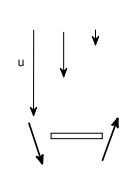
\includegraphics[scale=0.5]{Bilder/Ausrichtung_Partikeln}
\end{figure}
\end{frame}









